\begin{enumerate}
\item Construct a $\triangle ABC$ in which $CA = 6cm$ , $AB = 5cm$ and $BAC= 45\degree$. Then  construct a triangle whose sides are $\frac{3}{5}$ of the corresponding sides of $\triangle ABC$.
\item Prove that in a right angle triangle, the square of the hypotenuse is equal the sum of squares of the other two sides.
\item In \figref{fig:figure1}, $DE \parallel BC$, $ AD = 1 cm , BD = 2 cm$. What is the ratio of the area of $\triangle ABC$ to the area of $\triangle ADE$?
\begin{figure}[H]
			\centering
			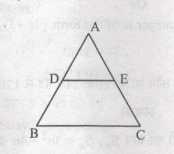
\includegraphics[width=\columnwidth]{figs/tri123.jpeg}
			\caption{}
			\label{fig:figure1}
			
			
		\end{figure} 
\item In \figref{fig:figure3}, angle $ACB = 90\degree$ and $CD \perp AB$, prove that $CD ^ 2 = BD \times AD$.
\begin{figure}[H]                                                            \centering
                        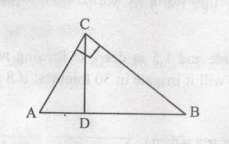
\includegraphics[width=\columnwidth]{figs/i3.jpeg}
			\caption{}
			\label{fig:figure3}
                \end{figure}
                
\item Construct a triangle $ABC$ with side $BC = 6 cm$, $\angle B=45\degree, \angle A= 105\degree$. Then construct another triangle whose sides are $\frac{3}{4}$ times the corresponding sides of the $\triangle ABC$
\item Prove that the ratio of the areas of two similar triangles is equal to the square of the ratio of their corresponding sides. 
\end{enumerate}
